\documentclass{standalone}
\usepackage{tikz}
\usetikzlibrary{patterns, positioning}
\usepackage[sfdefault]{ClearSans} %% option 'sfdefault' activates Clear Sans as the default text font
\usepackage[T1]{fontenc}

\begin{document}
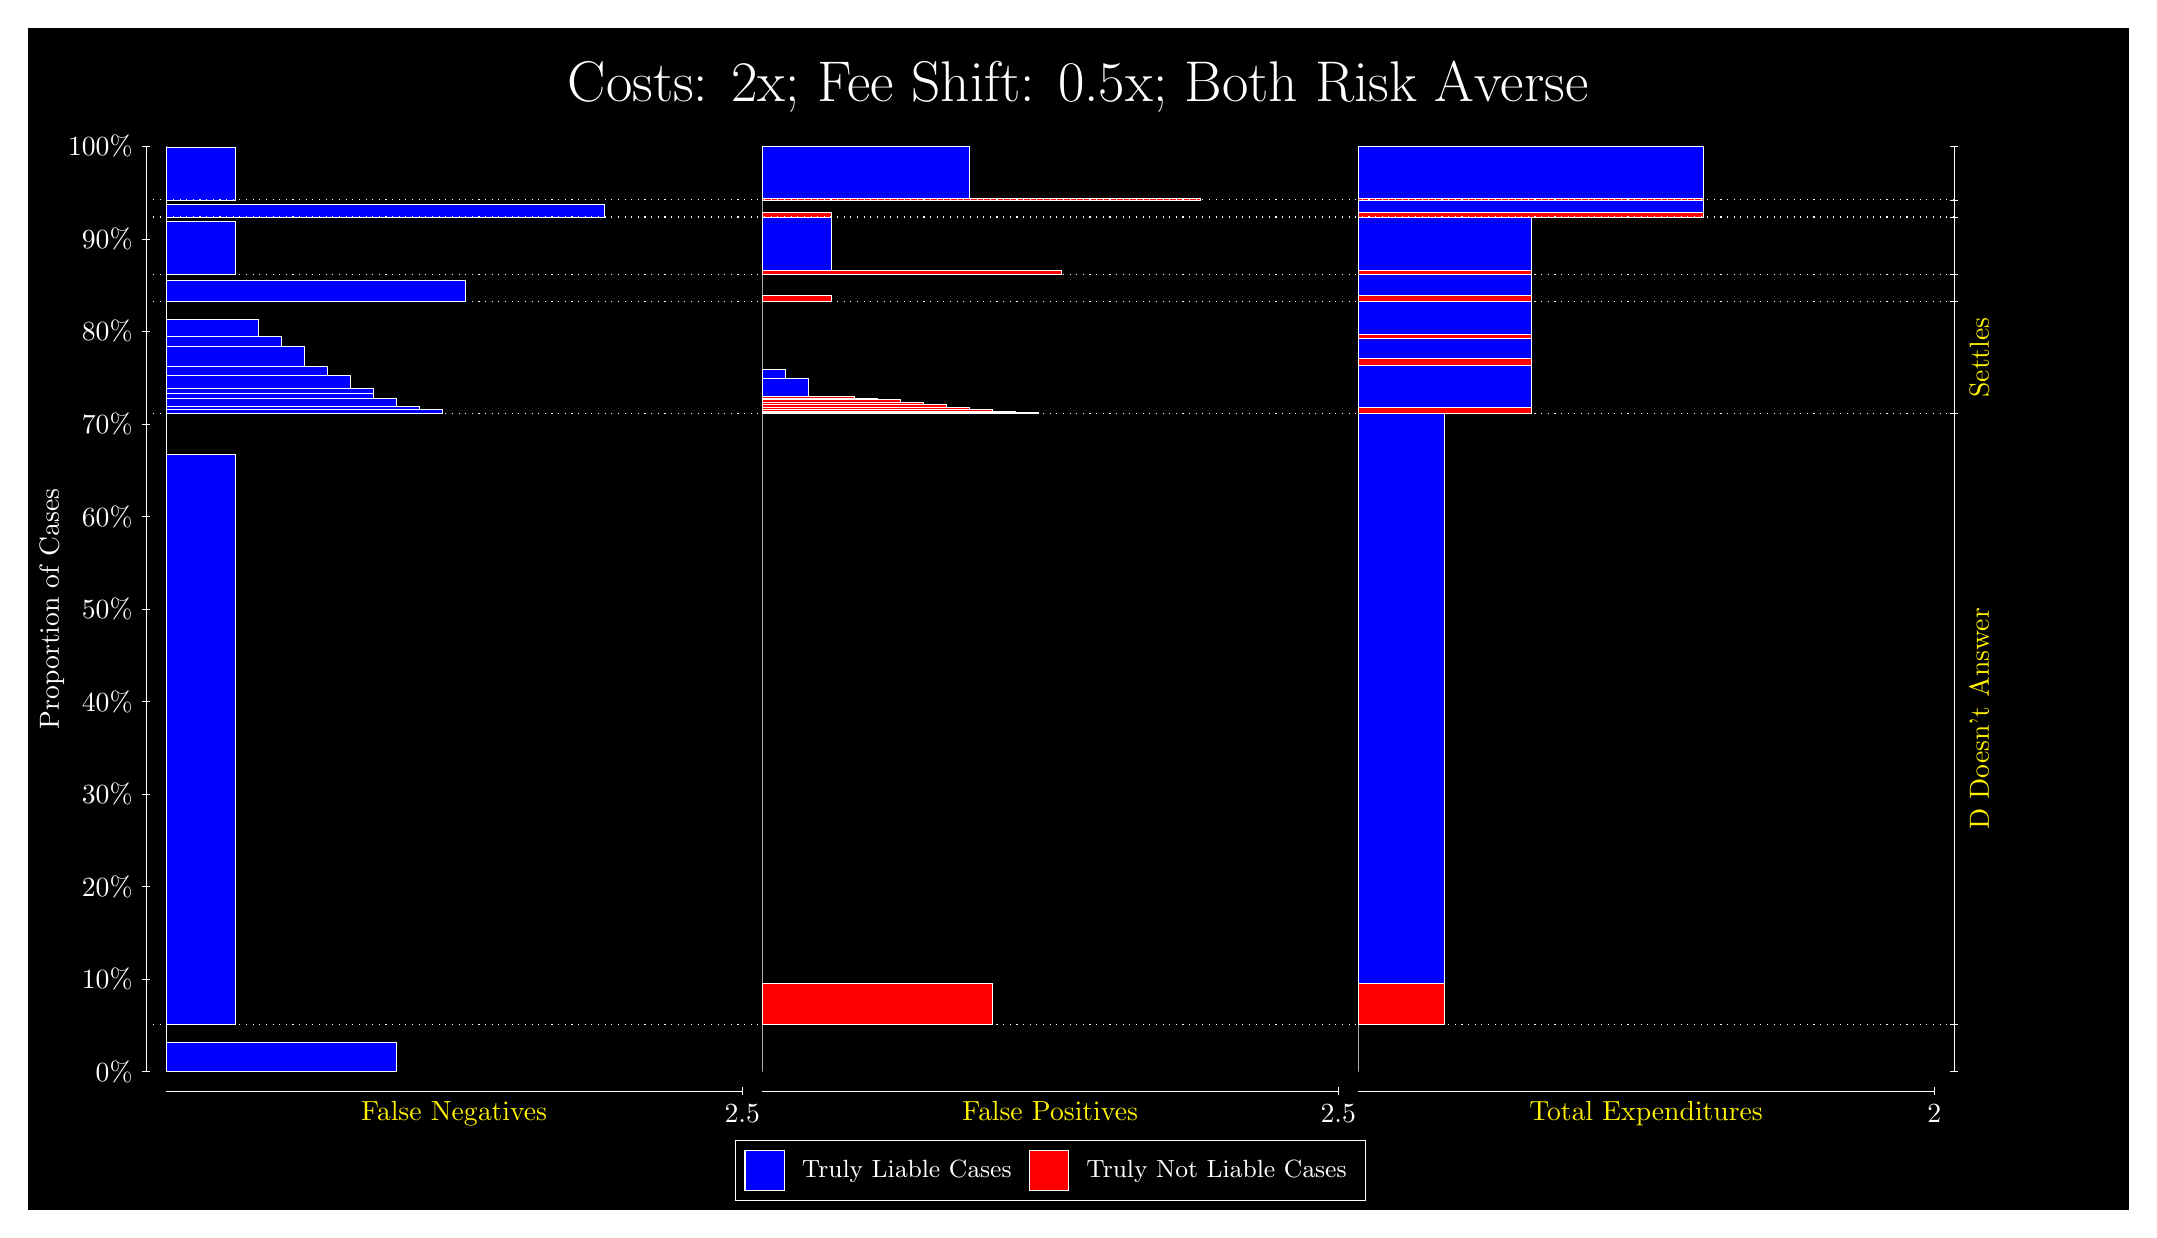
\begin{tikzpicture}
\draw[fill=black] (0,0) rectangle (26.667,15);
\draw[text=white] (0,13.5) rectangle (26.667,15) node[midway] {\huge Costs: 2x; Fee Shift: 0.5x; Both Risk Averse};
\draw[white, very thin] (1.5,1.75) -- (1.5,13.5);
\node[rotate=90, text=white, anchor=center] at (0.3, 7.625) {Proportion of Cases};
\draw[white, very thin] (1.45,1.75) -- (1.55,1.75);
\node[text=white, anchor=east] at (1.45, 1.75) {0\%};
\draw[white, very thin] (1.45,2.925) -- (1.55,2.925);
\node[text=white, anchor=east] at (1.45, 2.925) {10\%};
\draw[white, very thin] (1.45,4.1) -- (1.55,4.1);
\node[text=white, anchor=east] at (1.45, 4.1) {20\%};
\draw[white, very thin] (1.45,5.275) -- (1.55,5.275);
\node[text=white, anchor=east] at (1.45, 5.275) {30\%};
\draw[white, very thin] (1.45,6.45) -- (1.55,6.45);
\node[text=white, anchor=east] at (1.45, 6.45) {40\%};
\draw[white, very thin] (1.45,7.625) -- (1.55,7.625);
\node[text=white, anchor=east] at (1.45, 7.625) {50\%};
\draw[white, very thin] (1.45,8.8) -- (1.55,8.8);
\node[text=white, anchor=east] at (1.45, 8.8) {60\%};
\draw[white, very thin] (1.45,9.975) -- (1.55,9.975);
\node[text=white, anchor=east] at (1.45, 9.975) {70\%};
\draw[white, very thin] (1.45,11.15) -- (1.55,11.15);
\node[text=white, anchor=east] at (1.45, 11.15) {80\%};
\draw[white, very thin] (1.45,12.325) -- (1.55,12.325);
\node[text=white, anchor=east] at (1.45, 12.325) {90\%};
\draw[white, very thin] (1.45,13.5) -- (1.55,13.5);
\node[text=white, anchor=east] at (1.45, 13.5) {100\%};

\draw[white, very thin] (24.457,1.75) -- (24.457,13.5);
\draw[white, very thin] (24.407,1.75) -- (24.507,1.75);
\node[anchor=west] at (24.407, 1.75) {};
\draw[white, very thin] (24.407,2.348) -- (24.507,2.348);
\node[anchor=west] at (24.407, 2.348) {};
\draw[white, very thin] (24.407,10.107) -- (24.507,10.107);
\node[anchor=west] at (24.407, 10.107) {};
\draw[white, very thin] (24.407,11.527) -- (24.507,11.527);
\node[anchor=west] at (24.407, 11.527) {};
\draw[white, very thin] (24.407,11.872) -- (24.507,11.872);
\node[anchor=west] at (24.407, 11.872) {};
\draw[white, very thin] (24.407,12.603) -- (24.507,12.603);
\node[anchor=west] at (24.407, 12.603) {};
\draw[white, very thin] (24.407,12.819) -- (24.507,12.819);
\node[anchor=west] at (24.407, 12.819) {};
\draw[white, very thin] (24.407,13.5) -- (24.507,13.5);
\node[anchor=west] at (24.407, 13.5) {};

\draw[white, very thin, fill=blue] (1.75,1.75) rectangle (4.6775,2.1257);
\draw[white, very thin, fill=red] (1.75,2.1257) rectangle (1.75,2.348);
\draw[white, very thin, fill=blue] (1.75,2.348) rectangle (2.6283,9.5842);
\draw[white, very thin, fill=red] (1.75,9.5842) rectangle (1.75,10.107);
\draw[white, very thin, fill=blue] (1.75,10.107) rectangle (5.2631,10.155);
\draw[white, very thin, fill=blue] (1.75,10.155) rectangle (4.9703,10.199);
\draw[white, very thin, fill=blue] (1.75,10.199) rectangle (4.6775,10.306);
\draw[white, very thin, fill=blue] (1.75,10.306) rectangle (4.3848,10.359);
\draw[white, very thin, fill=blue] (1.75,10.359) rectangle (4.3848,10.421);
\draw[white, very thin, fill=blue] (1.75,10.421) rectangle (4.092,10.587);
\draw[white, very thin, fill=blue] (1.75,10.587) rectangle (3.7993,10.709);
\draw[white, very thin, fill=blue] (1.75,10.709) rectangle (3.5065,10.96);
\draw[white, very thin, fill=blue] (1.75,10.96) rectangle (3.2138,11.083);
\draw[white, very thin, fill=blue] (1.75,11.083) rectangle (2.921,11.307);
\draw[white, very thin, fill=red] (1.75,11.307) rectangle (1.75,11.527);
\draw[white, very thin, fill=blue] (1.75,11.527) rectangle (5.5558,11.796);
\draw[white, very thin, fill=red] (1.75,11.796) rectangle (1.75,11.872);
\draw[white, very thin, fill=blue] (1.75,11.872) rectangle (2.6283,12.547);
\draw[white, very thin, fill=red] (1.75,12.547) rectangle (1.75,12.603);
\draw[white, very thin, fill=blue] (1.75,12.603) rectangle (7.3123,12.759);
\draw[white, very thin, fill=red] (1.75,12.759) rectangle (1.75,12.819);
\draw[white, very thin, fill=blue] (1.75,12.819) rectangle (2.6283,13.483);
\draw[white, very thin, fill=red] (1.75,13.483) rectangle (1.75,13.5);
\draw[white, very thin, fill=red] (9.3189,1.75) rectangle (9.3189,1.9723);
\draw[white, very thin, fill=blue] (9.3189,1.9723) rectangle (9.3189,2.348);
\draw[white, very thin, fill=red] (9.3189,2.348) rectangle (12.246,2.8708);
\draw[white, very thin, fill=blue] (9.3189,2.8708) rectangle (9.3189,10.107);
\draw[white, very thin, fill=red] (9.3189,10.107) rectangle (12.832,10.12);
\draw[white, very thin, fill=red] (9.3189,10.12) rectangle (12.539,10.132);
\draw[white, very thin, fill=red] (9.3189,10.132) rectangle (12.246,10.156);
\draw[white, very thin, fill=red] (9.3189,10.156) rectangle (11.954,10.183);
\draw[white, very thin, fill=red] (9.3189,10.183) rectangle (11.661,10.222);
\draw[white, very thin, fill=red] (9.3189,10.222) rectangle (11.368,10.254);
\draw[white, very thin, fill=red] (9.3189,10.254) rectangle (11.075,10.289);
\draw[white, very thin, fill=red] (9.3189,10.289) rectangle (10.783,10.304);
\draw[white, very thin, fill=red] (9.3189,10.304) rectangle (10.49,10.327);
\draw[white, very thin, fill=blue] (9.3189,10.327) rectangle (9.9044,10.55);
\draw[white, very thin, fill=blue] (9.3189,10.55) rectangle (9.6116,10.674);
\draw[white, very thin, fill=blue] (9.3189,10.674) rectangle (9.3189,11.527);
\draw[white, very thin, fill=red] (9.3189,11.527) rectangle (10.197,11.603);
\draw[white, very thin, fill=blue] (9.3189,11.603) rectangle (9.3189,11.872);
\draw[white, very thin, fill=red] (9.3189,11.872) rectangle (13.125,11.928);
\draw[white, very thin, fill=blue] (9.3189,11.928) rectangle (10.197,12.603);
\draw[white, very thin, fill=red] (9.3189,12.603) rectangle (10.197,12.663);
\draw[white, very thin, fill=blue] (9.3189,12.663) rectangle (9.3189,12.819);
\draw[white, very thin, fill=red] (9.3189,12.819) rectangle (14.881,12.837);
\draw[white, very thin, fill=blue] (9.3189,12.837) rectangle (11.954,13.5);
\draw[white, very thin, fill=red] (16.888,1.75) rectangle (16.888,1.9723);
\draw[white, very thin, fill=blue] (16.888,1.9723) rectangle (16.888,2.348);
\draw[white, very thin, fill=red] (16.888,2.348) rectangle (17.986,2.8708);
\draw[white, very thin, fill=blue] (16.888,2.8708) rectangle (17.986,10.107);
\draw[white, very thin, fill=red] (16.888,10.107) rectangle (19.083,10.183);
\draw[white, very thin, fill=blue] (16.888,10.183) rectangle (19.083,10.724);
\draw[white, very thin, fill=red] (16.888,10.724) rectangle (19.083,10.807);
\draw[white, very thin, fill=blue] (16.888,10.807) rectangle (19.083,11.059);
\draw[white, very thin, fill=red] (16.888,11.059) rectangle (19.083,11.119);
\draw[white, very thin, fill=blue] (16.888,11.119) rectangle (19.083,11.527);
\draw[white, very thin, fill=red] (16.888,11.527) rectangle (19.083,11.603);
\draw[white, very thin, fill=blue] (16.888,11.603) rectangle (19.083,11.872);
\draw[white, very thin, fill=red] (16.888,11.872) rectangle (19.083,11.928);
\draw[white, very thin, fill=blue] (16.888,11.928) rectangle (19.083,12.603);
\draw[white, very thin, fill=red] (16.888,12.603) rectangle (21.279,12.663);
\draw[white, very thin, fill=blue] (16.888,12.663) rectangle (21.279,12.819);
\draw[white, very thin, fill=red] (16.888,12.819) rectangle (21.279,12.837);
\draw[white, very thin, fill=blue] (16.888,12.837) rectangle (21.279,13.5);
\draw[white, dotted] (1.5,2.348) -- (24.457,2.348);
\draw[white, dotted] (1.5,10.107) -- (24.457,10.107);
\draw[white, dotted] (1.5,11.527) -- (24.457,11.527);
\draw[white, dotted] (1.5,11.872) -- (24.457,11.872);
\draw[white, dotted] (1.5,12.603) -- (24.457,12.603);
\draw[white, dotted] (1.5,12.819) -- (24.457,12.819);
\draw[white, very thin] (1.75,1.5) -- (9.0689,1.5);
\node[text=yellow, anchor=north] at (5.4094, 1.5) {False Negatives};
\draw[white, very thin] (9.0689,1.45) -- (9.0689,1.55);
\node[text=white, anchor=north] at (9.0689, 1.45) {2.5};

\draw[white, very thin] (9.3189,1.5) -- (16.638,1.5);
\node[text=yellow, anchor=north] at (12.978, 1.5) {False Positives};
\draw[white, very thin] (16.638,1.45) -- (16.638,1.55);
\node[text=white, anchor=north] at (16.638, 1.45) {2.5};

\draw[white, very thin] (16.888,1.5) -- (24.207,1.5);
\node[text=yellow, anchor=north] at (20.547, 1.5) {Total Expenditures};
\draw[white, very thin] (24.207,1.45) -- (24.207,1.55);
\node[text=white, anchor=north] at (24.207, 1.45) {2};


\node[text=yellow, centered, rotate=90] at (24.777, 6.2275) {D Doesn't Answer};
\node[text=yellow, centered, rotate=90] at (24.777, 10.817) {Settles};





\draw (12.978300999999998,1.5) node[draw=none] (baseCoordinate) {};
\begin{scope}[align=center]
        \matrix[scale=0.5, draw=white, below=0.5cm of baseCoordinate, nodes={draw}, column sep=0.1cm]{
            \node[rectangle, draw, minimum width=0.5cm, minimum height=0.5cm, fill=blue] {}; &
            \node[draw=none, font=\small, text=white] (B) {Truly Liable Cases}; &
            \node[rectangle, draw, minimum width=0.5cm, minimum height=0.5cm, fill=red] {}; &
            \node[draw=none, font=\small, text=white] (B) {Truly Not Liable Cases}; \\
            };
\end{scope}

\end{tikzpicture}
\end{document}